\chapter{The Fifth of October} 

 \lettrine{I}{t} was about six o'clock in the evening; an opal-coloured light, through which an autumnal sun shed its golden rays, descended on the blue ocean. The heat of the day had gradually decreased, and a light breeze arose, seeming like the respiration of nature on awakening from the burning siesta of the south. A delicious zephyr played along the coasts of the Mediterranean, and wafted from shore to shore the sweet perfume of plants, mingled with the fresh smell of the sea. 

 A light yacht, chaste and elegant in its form, was gliding amidst the first dews of night over the immense lake, extending from Gibraltar to the Dardanelles, and from Tunis to Venice. The vessel resembled a swan with its wings opened towards the wind, gliding on the water. It advanced swiftly and gracefully, leaving behind it a glittering stretch of foam. By degrees the sun disappeared behind the western horizon; but as though to prove the truth of the fanciful ideas in heathen mythology, its indiscreet rays reappeared on the summit of every wave, as if the god of fire had just sunk upon the bosom of Amphitrite, who in vain endeavoured to hide her lover beneath her azure mantle. 

 The yacht moved rapidly on, though there did not appear to be sufficient wind to ruffle the curls on the head of a young girl. Standing on the prow was a tall man, of a dark complexion, who saw with dilating eyes that they were approaching a dark mass of land in the shape of a cone, which rose from the midst of the waves like the hat of a Catalan. 

 <Is that Monte Cristo?> asked the traveller, to whose orders the yacht was for the time submitted, in a melancholy voice. 

 <Yes, your excellency,> said the captain, <we have reached it.> 

 <We have reached it!> repeated the traveller in an accent of indescribable sadness. 

 Then he added, in a low tone, <Yes; that is the haven.> 

 And then he again plunged into a train of thought, the character of which was better revealed by a sad smile, than it would have been by tears. A few minutes afterwards a flash of light, which was extinguished instantly, was seen on the land, and the sound of firearms reached the yacht. 

 <Your excellency,> said the captain, <that was the land signal, will you answer yourself?> 

 <What signal?> 

 The captain pointed towards the island, up the side of which ascended a volume of smoke, increasing as it rose. 

 <Ah, yes,> he said, as if awaking from a dream. <Give it to me.> 

 The captain gave him a loaded carbine; the traveller slowly raised it, and fired in the air. Ten minutes afterwards, the sails were furled, and they cast anchor about a hundred fathoms from the little harbour. The gig was already lowered, and in it were four oarsmen and a coxswain. The traveller descended, and instead of sitting down at the stern of the boat, which had been decorated with a blue carpet for his accommodation, stood up with his arms crossed. The rowers waited, their oars half lifted out of the water, like birds drying their wings.  <Give way,> said the traveller. The eight oars fell into the sea simultaneously without splashing a drop of water, and the boat, yielding to the impulsion, glided forward. In an instant they found themselves in a little harbour, formed in a natural creek; the boat grounded on the fine sand. 

 <Will your excellency be so good as to mount the shoulders of two of our men, they will carry you ashore?> The young man answered this invitation with a gesture of indifference, and stepped out of the boat; the sea immediately rose to his waist. 

 <Ah, your excellency,> murmured the pilot, <you should not have done so; our master will scold us for it.> 

 The young man continued to advance, following the sailors, who chose a firm footing. Thirty strides brought them to dry land; the young man stamped on the ground to shake off the wet, and looked around for someone to show him his road, for it was quite dark. Just as he turned, a hand rested on his shoulder, and a voice which made him shudder exclaimed: 

 <Good-evening, Maximilian; you are punctual, thank you!> 

 <Ah, is it you, count?> said the young man, in an almost joyful accent, pressing Monte Cristo's hand with both his own. 

 <Yes; you see I am as exact as you are. But you are dripping, my dear fellow; you must change your clothes, as Calypso said to Telemachus. Come, I have a habitation prepared for you in which you will soon forget fatigue and cold.> 

 Monte Cristo perceived that the young man had turned around; indeed, Morrel saw with surprise that the men who had brought him had left without being paid, or uttering a word. Already the sound of their oars might be heard as they returned to the yacht. 

 <Oh, yes,> said the count, <you are looking for the sailors.> 

 <Yes, I paid them nothing, and yet they are gone.> 

 <Never mind that, Maximilian,> said Monte Cristo, smiling. <I have made an agreement with the navy, that the access to my island shall be free of all charge. I have made a bargain.> 

 Morrel looked at the count with surprise. <Count,> he said, <you are not the same here as in Paris.> 

 <How so?> 

 <Here you laugh.> The count's brow became clouded. 

 <You are right to recall me to myself, Maximilian,> he said; <I was delighted to see you again, and forgot for the moment that all happiness is fleeting.> 

 <Oh, no, no, count,> cried Maximilian, seizing the count's hands, <pray laugh; be happy, and prove to me, by your indifference, that life is endurable to sufferers. Oh, how charitable, kind, and good you are; you affect this gayety to inspire me with courage.> 

 <You are wrong, Morrel; I was really happy.> 

 <Then you forget me, so much the better.> 

 <How so?> 

 <Yes; for as the gladiator said to the emperor, when he entered the arena, <He who is about to die salutes you.>> 

 <Then you are not consoled?> asked the count, surprised. 

 <Oh,> exclaimed Morrel, with a glance full of bitter reproach, <do you think it possible that I could be?> 

 <Listen,> said the count. <Do you understand the meaning of my words? You cannot take me for a commonplace man, a mere rattle, emitting a vague and senseless noise. When I ask you if you are consoled, I speak to you as a man for whom the human heart has no secrets. Well, Morrel, let us both examine the depths of your heart. Do you still feel the same feverish impatience of grief which made you start like a wounded lion? Have you still that devouring thirst which can only be appeased in the grave? Are you still actuated by the regret which drags the living to the pursuit of death; or are you only suffering from the prostration of fatigue and the weariness of hope deferred? Has the loss of memory rendered it impossible for you to weep? Oh, my dear friend, if this be the case,—if you can no longer weep, if your frozen heart be dead, if you put all your trust in God, then, Maximilian, you are consoled—do not complain.> 

 <Count,> said Morrel, in a firm and at the same time soft voice, <listen to me, as to a man whose thoughts are raised to heaven, though he remains on earth; I come to die in the arms of a friend. Certainly, there are people whom I love. I love my sister Julie,—I love her husband Emmanuel; but I require a strong mind to smile on my last moments. My sister would be bathed in tears and fainting; I could not bear to see her suffer. Emmanuel would tear the weapon from my hand, and alarm the house with his cries. You, count, who are more than mortal, will, I am sure, lead me to death by a pleasant path, will you not?>

<My friend,> said the count, <I have still one doubt,—are you weak enough to pride yourself upon your sufferings?> 

 <No, indeed,—I am calm,> said Morrel, giving his hand to the count; <my pulse does not beat slower or faster than usual. No, I feel that I have reached the goal, and I will go no farther. You told me to wait and hope; do you know what you did, unfortunate adviser? I waited a month, or rather I suffered for a month! I did hope (man is a poor wretched creature), I did hope. What I cannot tell,—something wonderful, an absurdity, a miracle,—of what nature he alone can tell who has mingled with our reason that folly we call hope. Yes, I did wait—yes, I did hope, count, and during this quarter of an hour we have been talking together, you have unconsciously wounded, tortured my heart, for every word you have uttered proved that there was no hope for me. Oh, count, I shall sleep calmly, deliciously in the arms of death.> 

 Morrel uttered these words with an energy which made the count shudder. 

 <My friend,> continued Morrel, <you named the fifth of October as the end of the period of waiting,—today is the fifth of October,> he took out his watch, <it is now nine o'clock,—I have yet three hours to live.> 

 <Be it so,> said the count, <come.> Morrel mechanically followed the count, and they had entered the grotto before he perceived it. He felt a carpet under his feet, a door opened, perfumes surrounded him, and a brilliant light dazzled his eyes. Morrel hesitated to advance; he dreaded the enervating effect of all that he saw. Monte Cristo drew him in gently. 

 <Why should we not spend the last three hours remaining to us of life, like those ancient Romans, who when condemned by Nero, their emperor and heir, sat down at a table covered with flowers, and gently glided into death, amid the perfume of heliotropes and roses?> 

 Morrel smiled. <As you please,> he said; <death is always death,—that is forgetfulness, repose, exclusion from life, and therefore from grief.> 

 He sat down, and Monte Cristo placed himself opposite to him. They were in the marvellous dining-room before described, where the statues had baskets on their heads always filled with fruits and flowers. Morrel had looked carelessly around, and had probably noticed nothing. 

 <Let us talk like men,> he said, looking at the count. 

 <Go on!> 

 <Count,> said Morrel, <you are the epitome of all human knowledge, and you seem like a being descended from a wiser and more advanced world than ours.> 

 <There is something true in what you say,> said the count, with that smile which made him so handsome; <I have descended from a planet called grief.>  
 <I believe all you tell me without questioning its meaning; for instance, you told me to live, and I did live; you told me to hope, and I almost did so. I am almost inclined to ask you, as though you had experienced death, <is it painful to die?>> 

 Monte Cristo looked upon Morrel with indescribable tenderness. <Yes,> he said, <yes, doubtless it is painful, if you violently break the outer covering which obstinately begs for life. If you plunge a dagger into your flesh, if you insinuate a bullet into your brain, which the least shock disorders,—then certainly, you will suffer pain, and you will repent quitting a life for a repose you have bought at so dear a price.> 

 <Yes; I know that there is a secret of luxury and pain in death, as well as in life; the only thing is to understand it.> 

 <You have spoken truly, Maximilian; according to the care we bestow upon it, death is either a friend who rocks us gently as a nurse, or an enemy who violently drags the soul from the body. Some day, when the world is much older, and when mankind will be masters of all the destructive powers in nature, to serve for the general good of humanity; when mankind, as you were just saying, have discovered the secrets of death, then that death will become as sweet and voluptuous as a slumber in the arms of your beloved.> 

 <And if you wished to die, you would choose this death, count?> 

 <Yes.> 

 Morrel extended his hand. <Now I understand,> he said, <why you had me brought here to this desolate spot, in the midst of the ocean, to this subterranean palace; it was because you loved me, was it not, count? It was because you loved me well enough to give me one of those sweet means of death of which we were speaking; a death without agony, a death which allows me to fade away while pronouncing Valentine's name and pressing your hand.> 

 <Yes, you have guessed rightly, Morrel,> said the count, <that is what I intended.> 

 <Thanks; the idea that tomorrow I shall no longer suffer, is sweet to my heart.> 

 <Do you then regret nothing?> 

 <No,> replied Morrel. 

 <Not even me?> asked the count with deep emotion. Morrel's clear eye was for the moment clouded, then it shone with unusual lustre, and a large tear rolled down his cheek. 

 <What,> said the count, <do you still regret anything in the world, and yet die?> 

 <Oh, I entreat you,> exclaimed Morrel in a low voice, <do not speak another word, count; do not prolong my punishment.> 

 The count fancied that he was yielding, and this belief revived the horrible doubt that had overwhelmed him at the Château d'If. 

 <I am endeavouring,> he thought, <to make this man happy; I look upon this restitution as a weight thrown into the scale to balance the evil I have wrought. Now, supposing I am deceived, supposing this man has not been unhappy enough to merit happiness. Alas, what would become of me who can only atone for evil by doing good?>  Then he said aloud: <Listen, Morrel, I see your grief is great, but still you do not like to risk your soul.> Morrel smiled sadly. 

 <Count,> he said, <I swear to you my soul is no longer my own.> 

 <Maximilian, you know I have no relation in the world. I have accustomed myself to regard you as my son: well, then, to save my son, I will sacrifice my life, nay, even my fortune.> 

 <What do you mean?> 

 <I mean, that you wish to quit life because you do not understand all the enjoyments which are the fruits of a large fortune. Morrel, I possess nearly a hundred millions and I give them to you; with such a fortune you can attain every wish. Are you ambitious? Every career is open to you. Overturn the world, change its character, yield to mad ideas, be even criminal—but live.> 

 <Count, I have your word,> said Morrel coldly; then taking out his watch, he added, <It is half-past eleven.> 

 <Morrel, can you intend it in my house, under my very eyes?> 

 <Then let me go,> said Maximilian, <or I shall think you did not love me for my own sake, but for yours;> and he arose. 

 <It is well,> said Monte Cristo whose countenance brightened at these words; <you wish it—you are inflexible. Yes, as you said, you are indeed wretched and a miracle alone can cure you. Sit down, Morrel, and wait.> 

 Morrel obeyed; the count arose, and unlocking a closet with a key suspended from his gold chain, took from it a little silver casket, beautifully carved and chased, the corners of which represented four bending figures, similar to the Caryatides, the forms of women, symbols of the angels aspiring to heaven. 

 He placed the casket on the table; then opening it took out a little golden box, the top of which flew open when touched by a secret spring. This box contained an unctuous substance partly solid, of which it was impossible to discover the colour, owing to the reflection of the polished gold, sapphires, rubies, emeralds, which ornamented the box. It was a mixed mass of blue, red, and gold. 

 The count took out a small quantity of this with a gilt spoon, and offered it to Morrel, fixing a long steadfast glance upon him. It was then observable that the substance was greenish. 

 <This is what you asked for,> he said, <and what I promised to give you.> 

 <I thank you from the depths of my heart,> said the young man, taking the spoon from the hands of Monte Cristo. The count took another spoon, and again dipped it into the golden box. <What are you going to do, my friend?> asked Morrel, arresting his hand. 

 <Well, the fact is, Morrel, I was thinking that I too am weary of life, and since an opportunity presents itself\longdash> 

 <Stay!> said the young man. <You who love, and are beloved; you, who have faith and hope,—oh, do not follow my example. In your case it would be a crime. Adieu, my noble and generous friend, adieu; I will go and tell Valentine what you have done for me.> 

 And slowly, though without any hesitation, only waiting to press the count's hand fervently, he swallowed the mysterious substance offered by Monte Cristo. Then they were both silent. Ali, mute and attentive, brought the pipes and coffee, and disappeared. By degrees, the light of the lamps gradually faded in the hands of the marble statues which held them, and the perfumes appeared less powerful to Morrel. Seated opposite to him, Monte Cristo watched him in the shadow, and Morrel saw nothing but the bright eyes of the count. An overpowering sadness took possession of the young man, his hands relaxed their hold, the objects in the room gradually lost their form and colour, and his disturbed vision seemed to perceive doors and curtains open in the wall.  <Friend,> he cried, <I feel that I am dying; thanks!> 

 He made a last effort to extend his hand, but it fell powerless beside him. Then it appeared to him that Monte Cristo smiled, not with the strange and fearful expression which had sometimes revealed to him the secrets of his heart, but with the benevolent kindness of a father for a child. At the same time the count appeared to increase in stature, his form, nearly double its usual height, stood out in relief against the red tapestry, his black hair was thrown back, and he stood in the attitude of an avenging angel. Morrel, overpowered, turned around in the armchair; a delicious torpor permeated every vein. A change of ideas presented themselves to his brain, like a new design on the kaleidoscope. Enervated, prostrate, and breathless, he became unconscious of outward objects; he seemed to be entering that vague delirium preceding death. He wished once again to press the count's hand, but his own was immovable. He wished to articulate a last farewell, but his tongue lay motionless and heavy in his throat, like a stone at the mouth of a sepulchre. Involuntarily his languid eyes closed, and still through his eyelashes a well-known form seemed to move amid the obscurity with which he thought himself enveloped. 

 The count had just opened a door. Immediately a brilliant light from the next room, or rather from the palace adjoining, shone upon the room in which he was gently gliding into his last sleep. Then he saw a woman of marvellous beauty appear on the threshold of the door separating the two rooms. Pale, and sweetly smiling, she looked like an angel of mercy conjuring the angel of vengeance. 

 <Is it heaven that opens before me?> thought the dying man; <that angel resembles the one I have lost.> 

 Monte Cristo pointed out Morrel to the young woman, who advanced towards him with clasped hands and a smile upon her lips. 

 <Valentine, Valentine!> he mentally ejaculated; but his lips uttered no sound, and as though all his strength were centred in that internal emotion, he sighed and closed his eyes. Valentine rushed towards him; his lips again moved. 

 <He is calling you,> said the count; <he to whom you have confided your destiny—he from whom death would have separated you, calls you to him. Happily, I vanquished death. Henceforth, Valentine, you will never again be separated on earth, since he has rushed into death to find you. Without me, you would both have died. May God accept my atonement in the preservation of these two existences!> 

 Valentine seized the count's hand, and in her irresistible impulse of joy carried it to her lips.  <Oh, thank me again!> said the count; <tell me till you are weary, that I have restored you to happiness; you do not know how much I require this assurance.> 

 <Oh, yes, yes, I thank you with all my heart,> said Valentine; <and if you doubt the sincerity of my gratitude, oh, then, ask Haydée! ask my beloved sister Haydée, who ever since our departure from France, has caused me to wait patiently for this happy day, while talking to me of you.> 

 <You then love Haydée?> asked Monte Cristo with an emotion he in vain endeavoured to dissimulate. 

 <Oh, yes, with all my soul.> 

 <Well, then, listen, Valentine,> said the count; <I have a favour to ask of you.> 

 <Of me? Oh, am I happy enough for that?> 

 <Yes; you have called Haydée your sister,—let her become so indeed, Valentine; render her all the gratitude you fancy that you owe to me; protect her, for> (the count's voice was thick with emotion) <henceforth she will be alone in the world.> 

 <Alone in the world!> repeated a voice behind the count, <and why?> 

 Monte Cristo turned around; Haydée was standing pale, motionless, looking at the count with an expression of fearful amazement. 

 <Because tomorrow, Haydée, you will be free; you will then assume your proper position in society, for I will not allow my destiny to overshadow yours. Daughter of a prince, I restore to you the riches and name of your father.> 

 Haydée became pale, and lifting her transparent hands to heaven, exclaimed in a voice stifled with tears, <Then you leave me, my lord?> 

 <Haydée, Haydée, you are young and beautiful; forget even my name, and be happy.> 

 <It is well,> said Haydée; <your order shall be executed, my lord; I will forget even your name, and be happy.> And she stepped back to retire. 

 <Oh, heavens,> exclaimed Valentine, who was supporting the head of Morrel on her shoulder, <do you not see how pale she is? Do you not see how she suffers?> 

 Haydée answered with a heartrending expression, 

 <Why should he understand this, my sister? He is my master, and I am his slave; he has the right to notice nothing.> 

 The count shuddered at the tones of a voice which penetrated the inmost recesses of his heart; his eyes met those of the young girl and he could not bear their brilliancy. 

 <Oh, heavens,> exclaimed Monte Cristo, <can my suspicions be correct? Haydée, would it please you not to leave me?> 

 <I am young,> gently replied Haydée; <I love the life you have made so sweet to me, and I should be sorry to die.> 

 <You mean, then, that if I leave you, Haydée\longdash> 

 <I should die; yes, my lord.> 

 <Do you then love me?> 

 <Oh, Valentine, he asks if I love him. Valentine, tell him if you love Maximilian.> 

 The count felt his heart dilate and throb; he opened his arms, and Haydée, uttering a cry, sprang into them. 

 <Oh, yes,> she cried, <I do love you! I love you as one loves a father, brother, husband! I love you as my life, for you are the best, the noblest of created beings!>

<Let it be, then, as you wish, sweet angel; God has sustained me in my struggle with my enemies, and has given me this reward; he will not let me end my triumph in suffering; I wished to punish myself, but he has pardoned me. Love me then, Haydée! Who knows? perhaps your love will make me forget all that I do not wish to remember.> 

 <What do you mean, my lord?> 

 <I mean that one word from you has enlightened me more than twenty years of slow experience; I have but you in the world, Haydée; through you I again take hold on life, through you I shall suffer, through you rejoice.> 

 <Do you hear him, Valentine?> exclaimed Haydée; <he says that through me he will suffer—through \textit{me}, who would yield my life for his.> 

 The count withdrew for a moment. <Have I discovered the truth?> he said; <but whether it be for recompense or punishment, I accept my fate. Come, Haydée, come!> and throwing his arm around the young girl's waist, he pressed the hand of Valentine, and disappeared.  An hour had nearly passed, during which Valentine, breathless and motionless, watched steadfastly over Morrel. At length she felt his heart beat, a faint breath played upon his lips, a slight shudder, announcing the return of life, passed through the young man's frame. At length his eyes opened, but they were at first fixed and expressionless; then sight returned, and with it feeling and grief. 

 <Oh,> he cried, in an accent of despair, <the count has deceived me; I am yet living;> and extending his hand towards the table, he seized a knife. 

 <Dearest,> exclaimed Valentine, with her adorable smile, <awake, and look at me!> Morrel uttered a loud exclamation, and frantic, doubtful, dazzled, as though by a celestial vision, he fell upon his knees. 

 The next morning at daybreak, Valentine and Morrel were walking arm-in-arm on the seashore, Valentine relating how Monte Cristo had appeared in her room, explained everything, revealed the crime, and, finally, how he had saved her life by enabling her to simulate death. 

 They had found the door of the grotto opened, and gone forth; on the azure dome of heaven still glittered a few remaining stars. 

 Morrel soon perceived a man standing among the rocks, apparently awaiting a sign from them to advance, and pointed him out to Valentine. 

 <Ah, it is Jacopo,> she said, <the captain of the yacht;> and she beckoned him towards them. 

 <Do you wish to speak to us?> asked Morrel. 

 <I have a letter to give you from the count.> 

 <From the count!> murmured the two young people. 

 <Yes; read it.>  Morrel opened the letter, and read: 

\begin{mail}{}{My Dear Maximilian,}

There is a felucca for you at anchor. Jacopo will carry you to Leghorn, where Monsieur Noirtier awaits his granddaughter, whom he wishes to bless before you lead her to the altar. All that is in this grotto, my friend, my house in the Champs-Élysées, and my château at Tréport, are the marriage gifts bestowed by Edmond Dantès upon the son of his old master, Morrel. Mademoiselle de Villefort will share them with you; for I entreat her to give to the poor the immense fortune reverting to her from her father, now a madman, and her brother who died last September with his mother. Tell the angel who will watch over your future destiny, Morrel, to pray sometimes for a man, who, like Satan, thought himself for an instant equal to God, but who now acknowledges with Christian humility that God alone possesses supreme power and infinite wisdom. Perhaps those prayers may soften the remorse he feels in his heart. As for you, Morrel, this is the secret of my conduct towards you. There is neither happiness nor misery in the world; there is only the comparison of one state with another, nothing more. He who has felt the deepest grief is best able to experience supreme happiness. We must have felt what it is to die, Morrel, that we may appreciate the enjoyments of living. 

Live, then, and be happy, beloved children of my heart, and never forget that until the day when God shall deign to reveal the future to man, all human wisdom is summed up in these two words,—<\textit{Wait and hope}.>
\closeletter[Your friend,]{Edmond Dantès,\\ \textit{Count of Monte Cristo}.}  
\end{mail}

During the perusal of this letter, which informed Valentine for the first time of the madness of her father and the death of her brother, she became pale, a heavy sigh escaped from her bosom, and tears, not the less painful because they were silent, ran down her cheeks; her happiness cost her very dear. 

 Morrel looked around uneasily. 

 <But,> he said, <the count's generosity is too overwhelming; Valentine will be satisfied with my humble fortune. Where is the count, friend? Lead me to him.> 

 Jacopo pointed towards the horizon. 

 <What do you mean?> asked Valentine. <Where is the count?—where is Haydée?> 

 <Look!> said Jacopo. 

 The eyes of both were fixed upon the spot indicated by the sailor, and on the blue line separating the sky from the Mediterranean Sea, they perceived a large white sail. 

 <Gone,> said Morrel; <gone!—adieu, my friend—adieu, my father!> 

 <Gone,> murmured Valentine; <adieu, my sweet Haydée—adieu, my sister!> 

 <Who can say whether we shall ever see them again?> said Morrel with tearful eyes. 

 <Darling,> replied Valentine, `has not the count just told us that all human wisdom is summed up in two words: 

\begin{quote}
\textit{Wait and hope} (Fac et spera)!'
\end{quote}

\vfill
\centerline{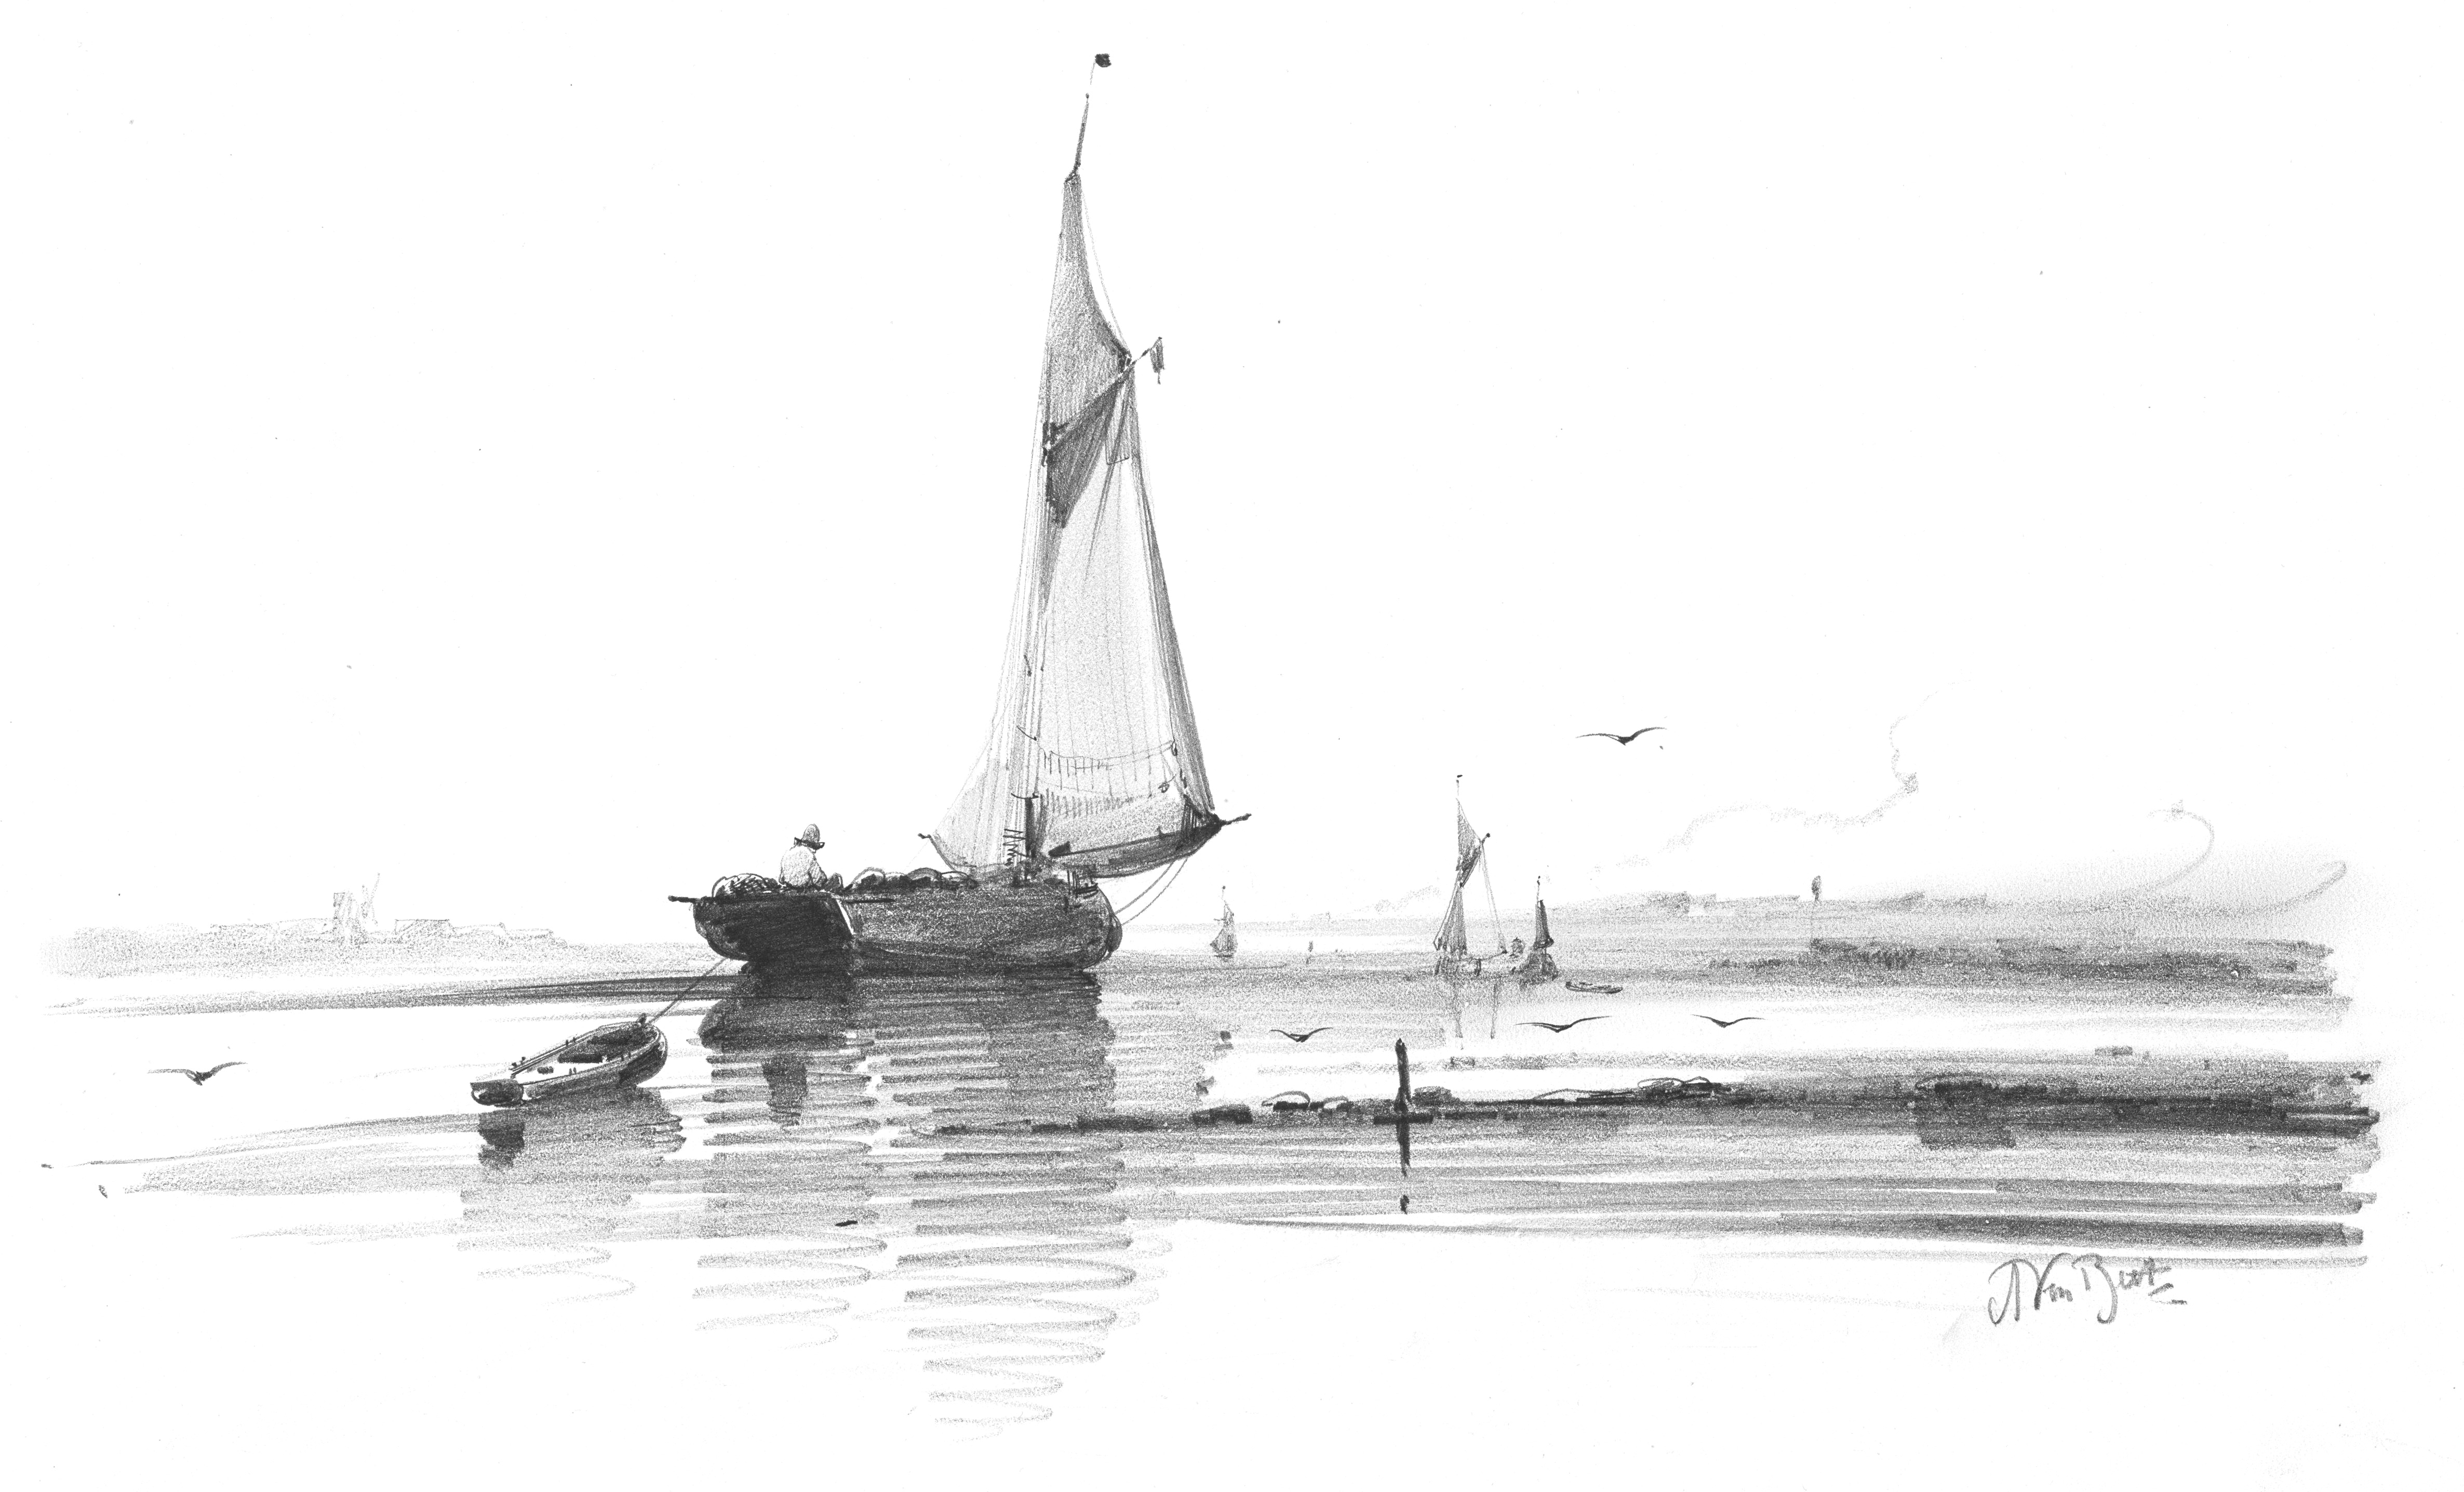
\includegraphics[width=\basicwidth]{sailboat}}
\vfill